En este apéndice se presenta el análisis detallado de los resultados obtenidos durante la fase de optimización de hiperparámetros para cada modelo y dataset.

\section{Modelos entrenados con UNSW-NB15}

\subsection{Random Forest}

Para el modelo de Random Forest, utilizando Optuna, se han obtenido los siguientes resultados como frontera de Pareto:

\begin{figure}[H]
    \centering
    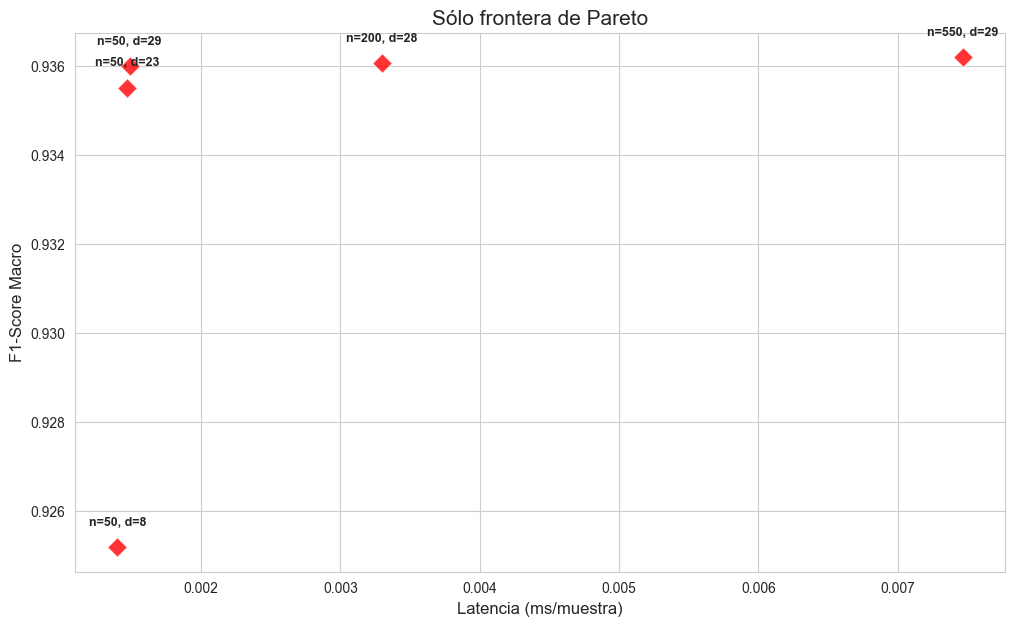
\includegraphics[width=0.8\textwidth]{images/PARETO_RF.png}
    \caption{Frontera de Pareto - Random Forest}
    \label{fig:pareto_rf}
\end{figure}

Hemos visto cómo reaccionan en test los modelos con los siguientes hiperparámetros elegidos:

\begin{enumerate}
    \item (50, 23) 
    \item (100, 29) 
    \item (200, 28) 
    \item (550, 29)
\end{enumerate}

Los resultados son los siguientes:

\begin{table}[H]
    \centering
    \begin{tabular}{|l|c|c|c|c|c|}
        \hline
        \textbf{Perfil} & \textbf{n\_estimators} & \textbf{max\_depth} & \textbf{F1\_Test} & \textbf{Accuracy\_Test} & \textbf{Latencia (ms)} \\
        \hline
        Candidato 1 & 50 & 23 & 0.885392 & 0.888622 & 0.001516 \\
        \hline
        Candidato 2 & 50 & 29 & 0.873085 & 0.877411 & 0.001486 \\
        \hline
        Candidato 3 & 200 & 28 & 0.876276 & 0.880338 & 0.003443 \\
        \hline
        Candidato 4 & 550 & 29 & 0.87463 & 0.878881 & 0.007078 \\
        \hline
    \end{tabular}
    \caption{Comparativa final de modelos Random Forest en el set de test}
    \label{tab:rf_comparison}
\end{table}

El \textbf{Candidato 1} no solo es el más preciso, sino también uno de los más rápidos, con una latencia de 0,0015 ms por muestra.

\subsection{XGBoost}

A continuaci\'on se muestran los resultados obtenidos por XGBoost:
\begin{figure}[H]
    \centering
    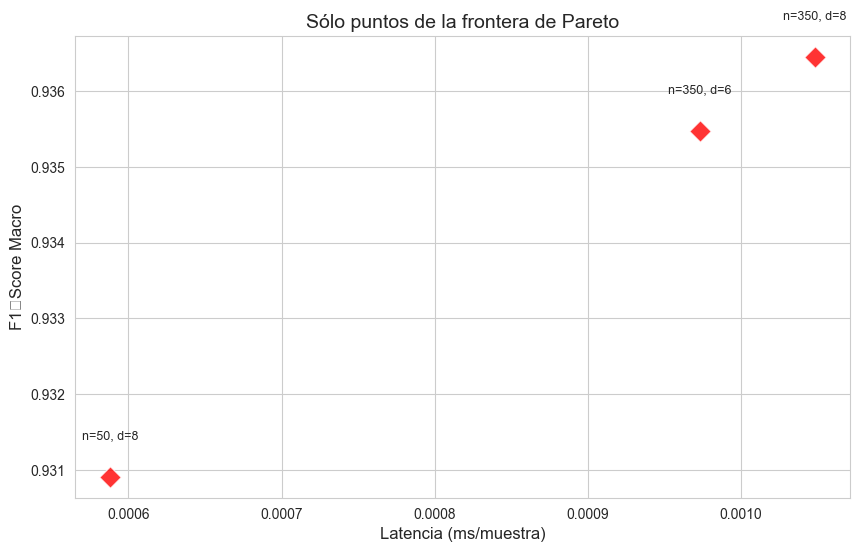
\includegraphics[width=0.8\textwidth]{images/PARETO_XGBOOST.png}
    \caption{Frontera de Pareto - XGBoost}
    \label{fig:pareto_xgboost}
\end{figure}

Hemos selecciondo las 3 combinaciones de la frontera de Pareto para testarlas:

\begin{enumerate}
    \item (350, 12) 
    \item (200, 11) 
    \item (350, 7) 
    \item (250, 8) 
    \item (100, 11) 
\end{enumerate}

Los resultados son los siguientes:

\begin{table}[H]
    \centering
    \begin{tabular}{|l|c|c|c|c|c|}
        \hline
        \textbf{Perfil} & \textbf{n\_estimators} & \textbf{max\_depth} & \textbf{F1\_Test} & \textbf{Accuracy\_Test} & \textbf{Latencia (ms)} \\
        \hline
        Candidato 1 & 350 & 12 & 0.858299 & 0.864378 & 0.000501 \\
        \hline
        Candidato 2 & 200 & 11 & 0.857905 & 0.864111 & 0.000418 \\
        \hline
        Candidato 3 & 350 & 7 & 0.856623 & 0.863152 & 0.000561 \\
        \hline
        Candidato 4 & 250 & 8 & 0.856923 & 0.863322 & 0.000543 \\
        \hline
        Candidato 5 & 100 & 11 & 0.857487 & 0.86388 & 0.000443 \\
        \hline
    \end{tabular}
    \caption{Comparativa final de modelos XGBoost en el set de test}
    \label{tab:xgboost_comparison}
\end{table}

Nos quedamos con el \textbf{Candidato 2}, que ofrece un excelente equilibrio entre calidad y coste.

\subsection{LightGBM}

LightGBM ha sido entrenado con GPU, obteniendo la siguiente frontera de Pareto:
\begin{figure}[H]
    \centering
    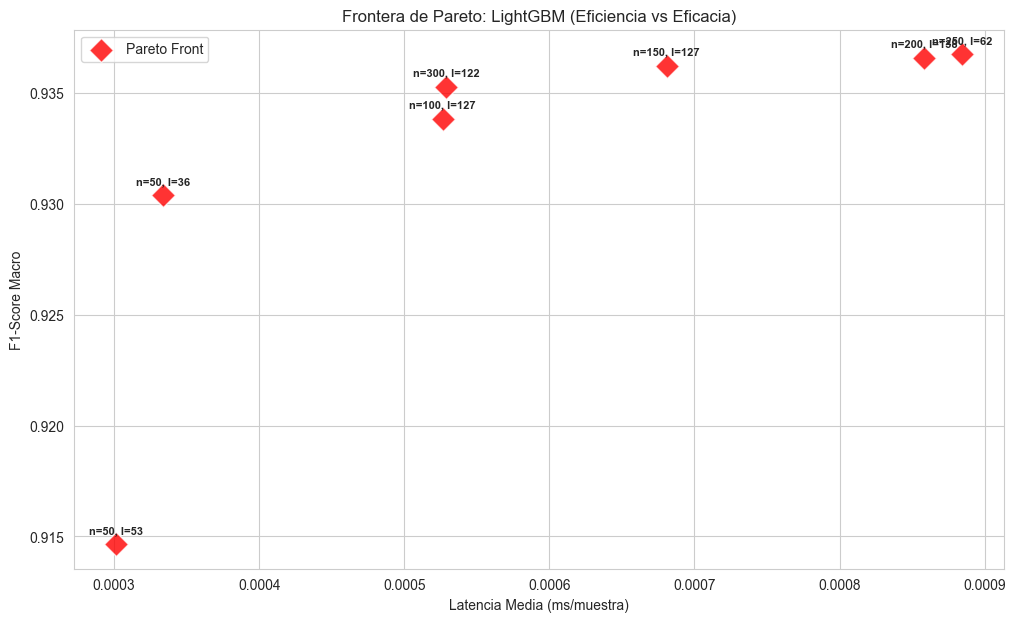
\includegraphics[width=0.8\textwidth]{images/PARETO_LIGHTGBM.png}
    \caption{Frontera de Pareto - LightGBM}
    \label{fig:pareto_lightgbm}
\end{figure}

Entre los diferentes puntos de la frontera de Pareto, se han seleccionado los siguientes para su evaluación en el set de test:
\begin{enumerate}
    \item (350, 68, 9) 
    \item (450, 29, 12) 
    \item (150, 90, 12) 
    \item (100, 145, 12) 
    \item (100, 122, 7) 
\end{enumerate}

Los resultados obtenidos en el set de test son los siguientesss:

\begin{table}[H]
    \centering
    \begin{tabular}{|l|c|c|c|c|c|c|}
        \hline
        \textbf{Perfil} & \textbf{n\_estimators} & \textbf{num\_leaves} & \textbf{max\_depth} & \textbf{F1\_Test} & \textbf{Accuracy\_Test} & \textbf{Latencia (ms)} \\
        \hline
        Candidato 1 & 350 & 68 & 9 & 0.861467 & 0.867354 & 0.000371 \\
        \hline
        Candidato 2 & 450 & 29 & 12 & 0.860196 & 0.86631 & 0.00036 \\
        \hline
        Candidato 3 & 150 & 90 & 12 & 0.860457 & 0.866552 & 0.0002 \\
        \hline
        Candidato 4 & 100 & 145 & 12 & 0.859564 & 0.865775 & 0.000159 \\
        \hline
        Candidato 5 & 100 & 122 & 7 & 0.852491 & 0.859654 & 0.000137 \\
        \hline

    \end{tabular}
    \caption{Comparativa final de modelos LightGBM en el set de test}
    \label{tab:lightgbm_comparison}
\end{table}

Si tuviéramos que quedarnos con un único modelo, nos quedamos con el \textbf{Candidato 4}. 

\subsection{CatBoost}

La frontera de Pareto obtenida para CatBoost con el dataset UNSW-NB15 es la siguiente:

\begin{figure}[H]
    \centering
    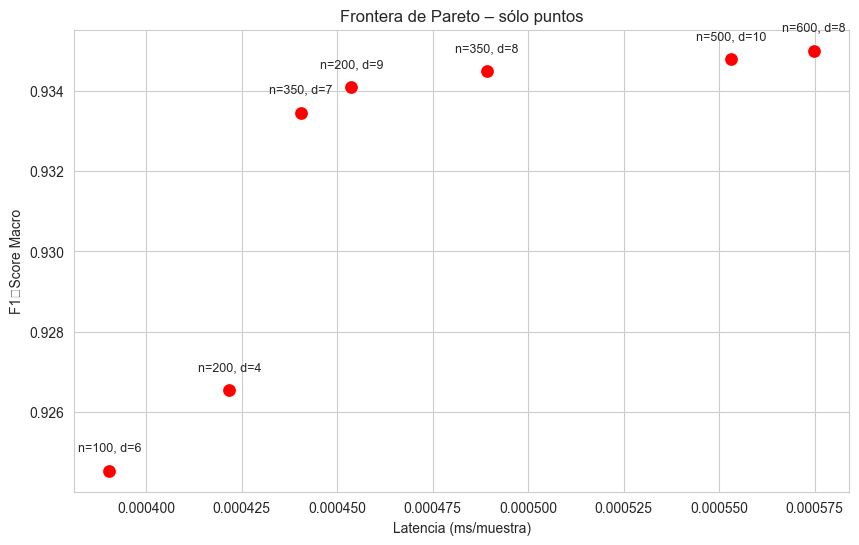
\includegraphics[width=0.8\textwidth]{images/PARETO_CATBOOST.png}
    \caption{Frontera de Pareto - CatBoost}
    \label{fig:pareto_catboost}
\end{figure}

Entre los diferentes puntos de la frontera de Pareto, se han seleccionado los siguientes para su evaluación en el set de test:

\begin{samepage}
\begin{enumerate}[nosep]
    \item (200, 4)
    \item (350, 7)
    \item (200, 9)
    \item (350, 8)
    \item (500, 10)
\end{enumerate}
\end{samepage}

Los resultados obtenidos en el set de test son los siguientes:

\begin{table}[H]
    \centering
    \begin{tabular}{|l|c|c|c|c|c|}
        \hline
        \textbf{Perfil} & \textbf{n\_estimators} & \textbf{max\_depth} & \textbf{F1\_Test} & \textbf{Accuracy\_Test} & \textbf{Latencia (ms)} \\
        \hline
        Candidato 1 & 200 & 4 & 0.828623 & 0.838957 & 0.000298 \\
        \hline
        Candidato 2 & 350 & 7 & 0.854301 & 0.861135 & 0.00044 \\
        \hline
        Candidato 3 & 200 & 9 & 0.85276 & 0.859787 & 0.000477 \\
        \hline
        Candidato 4 & 350 & 8 & 0.855648 & 0.862277 & 0.000489 \\
        \hline
        Candidato 5 & 500 & 10 & 0.85702 & 0.863419 & 0.000375 \\
        \hline
    \end{tabular}
    \caption{Comparativa final de modelos CatBoost en el set de test} 
    \label{tab:catboost_comparison}
\end{table}

El dato más revelador de la tabla es la latencia del \textbf{Candidato 5} (n=500, d=10). 
A pesar de ser el modelo más masivo y profundo de los evaluados, presenta una latencia de 0.000375 ms, siendo más rápido que modelos teóricamente más sencillos como el Candidato 4 (n=350, d=8, con 0.000489 ms). 

%------------------------------------------------------------------------------------
%------------------------------------------------------------------------------------
%------------------------------------------------------------------------------------
    
\subsection{SVM}

La gráfica de la frontera de Pareto obtenida para SVM:

\begin{figure}[H]
    \centering
    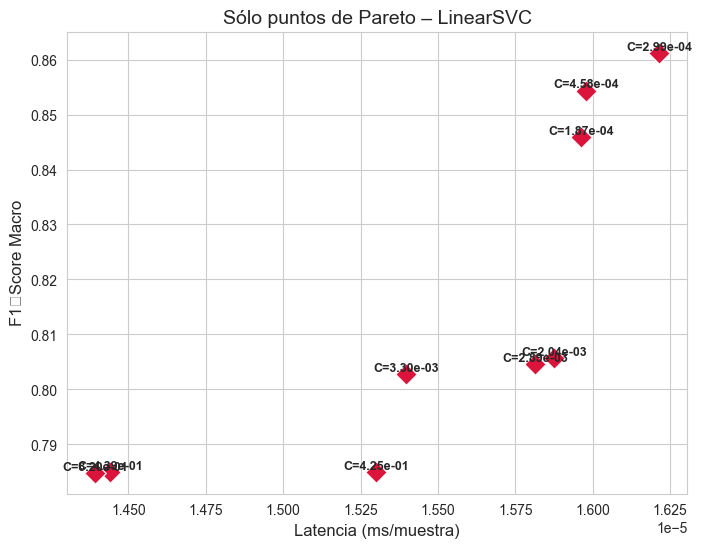
\includegraphics[width=0.8\textwidth]{images/PARETO_SVM.png}
    \caption{Frontera de Pareto - SVM}
    \label{fig:pareto_svm}
\end{figure}

Los resultados obtenidos en el set de test para los modelos seleccionados de la frontera de Pareto son los siguientes:

\begin{table}[H]
    \centering
    \begin{tabular}{|l|c|c|c|c|}
        \hline
        \textbf{Perfil} & \textbf{C} & \textbf{F1\_Test} & \textbf{Accuracy\_Test} & \textbf{Latencia (ms)} \\
        \hline
        Candidato 1 & 0.000299 & 0.708654 & 0.735461 & 0.000081 \\
        \hline
        Candidato 2 & 0.000458 & 0.692147 & 0.722987 & 0.000093 \\
        \hline
        Candidato 3 & 0.000187 & 0.709219 & 0.736105 & 0.000018 \\
        \hline
        Candidato 4 & 0.002037 & 0.649204 & 0.692003 & 0.000019 \\
        \hline
        Candidato 5 & 0.002889 & 0.648003 & 0.691104 & 0.000018 \\
        \hline
    \end{tabular}
    \caption{Comparativa final de modelos SVM en el set de test}
    \label{tab:svm_comparison}
\end{table}

A diferencia de los modelos basados en árboles (RF, XGBoost, LightGBM) que superaban holgadamente el 85\% de F1-Score, LinearSVC se estanca en un máximo de 0.7092 (Candidato 3). Esta drástica caída de rendimiento demuestra empíricamente que las intrusiones de red no son linealmente separables en este espacio de características.

Dentro de las limitaciones del enfoque lineal, el \textbf{Candidato 3} (C=0.000187) es el ganador absoluto e indiscutible.

\subsection{MLP}

La gráfica de la frontera de Pareto obtenida para MLP es la siguiente:

\begin{figure}[H]
    \centering
    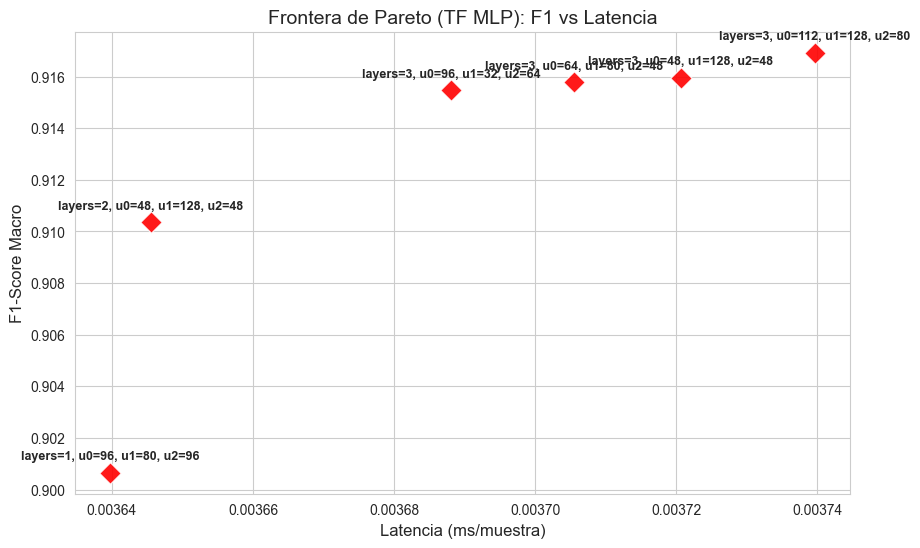
\includegraphics[width=0.8\textwidth]{images/PARETO_MLP.png}
    \caption{Frontera de Pareto - MLP}
    \label{fig:pareto_mlp}
\end{figure}

Ahora mostramos los resultados obtenidos en el set de test para los modelos seleccionados de la frontera de Pareto:

\begin{table}[H]
    \centering
    \resizebox{\textwidth}{!}{
    \begin{tabular}{|l|c|c|c|c|c|c|c|}
        \hline
        \textbf{Perfil} & \textbf{n\_layers} & \textbf{n\_units\_l0} & \textbf{n\_units\_l1} & \textbf{n\_units\_l2} & \textbf{F1\_Test} & \textbf{Accuracy\_Test} & \textbf{Latencia (ms)} \\
        \hline
        Candidato 1 & 3 & 96 & 80 & 96 & 0.777448 & 0.797017 & 0.00159 \\
        \hline
        Candidato 2 & 3 & 48 & 128 & 48 & 0.758004 & 0.781397 & 0.001505 \\
        \hline
        Candidato 3 & 3 & 64 & 80 & 48 & 0.782289 & 0.800515 & 0.001505 \\
        \hline
        Candidato 4 & 3 & 96 & 32 & 64 & 0.786982 & 0.804147 & 0.001421 \\
        \hline
    \end{tabular}
    }
    \caption{Comparativa final de modelos MLP en el set de test}
    \label{tab:mlp_comparison}
\end{table}

Nos quedamos con el \textbf{Candidato 4}, que ofrece el mejor rendimiento (F1-Score de 0.7869) y una latencia de inferencia de 0.001421 ms, lo que lo posiciona como un modelo competitivo dentro de los modelos no lineales, aunque aún por debajo de los basados en árboles.

% \subsection{LSTM}

% Con LSTM, la gráfica de la frontera de Pareto obtenida es la siguiente:

% \begin{figure}[H]
%     \centering
%     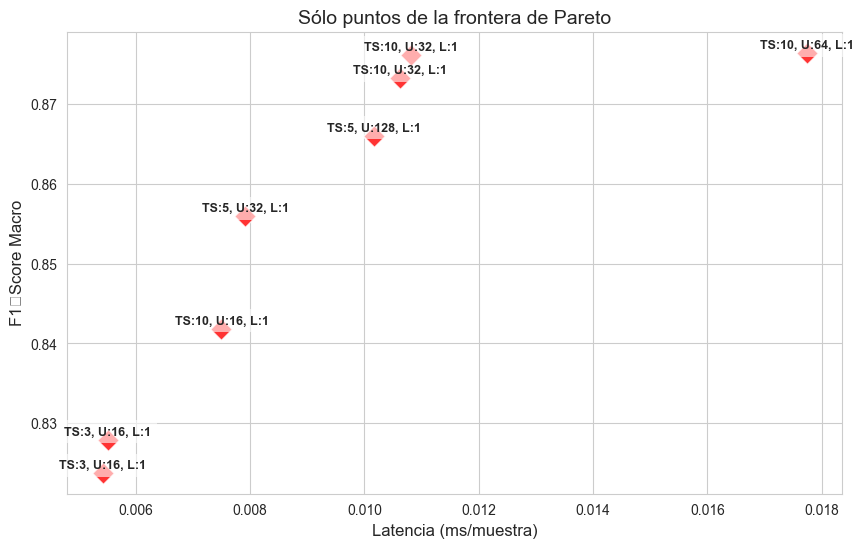
\includegraphics[width=0.8\textwidth]{images/PARETO_LSTM.png}
%     \caption{Frontera de Pareto - LSTM}
%     \label{fig:pareto_lstm}
% \end{figure}

% Los resultados obtenidos en el set de test para los modelos seleccionados de la frontera de Pareto son los siguientes:

% \begin{table}[H]
%     \centering
%     \begin{tabular}{|l|c|c|c|c|c|c|c|}
%         \hline
%         \textbf{Perfil} & \textbf{TS} & \textbf{Units} & \textbf{Layers}  & \textbf{F1\_Test} & \textbf{Accuracy\_Test} & \textbf{Latencia (ms)} \\
%         \hline
%         Candidato 1 & 10 & 32 & 1 & 0.918214 & 0.920569 & 0.008549 \\
%         \hline
%         Candidato 2 & 5 & 128 & 1 & 0.893188 & 0.897131 & 0.007129 \\
%         \hline
%         Candidato 3 & 5 & 32 & 1 & 0.886394 & 0.890766 & 0.004702 \\
%         \hline
%         Candidato 4 & 10 & 64 & 1 & 0.913959 & 0.916597 & 0.014846 \\
%         \hline
%     \end{tabular}
%     \caption{Comparativa final de modelos LSTM en el set de test}
%     \label{tab:lstm_comparison}
% \end{table}

% Nos quedamos con el \textbf{Candidato 1}, que ofrece un excelente rendimiento (F1-Score de 0.9182) pero con una latencia de inferencia de 0.008549 ms, lo que lo posiciona como un modelo muy preciso pero con un coste computacional elevado si lo comparamos con los modelos de árboles.
% Los modelos con TS: 10 (Candidatos 1 y 4) superan holgadamente la barrera del 0.91 de F1.
% Los modelos con TS: 5 (Candidatos 2 y 3) se quedan en el rango de 0.88 - 0.89.
% Incluso si le das 128 unidades a un modelo con TS:5 (Candidato 2), no logra alcanzar el rendimiento de un modelo con solo 32 unidades pero con TS:10. Conclusión: El modelo necesita "ver" más atrás en el tiempo (TS:10) para entender correctamente el patrón, y añadir más "neuronas" (unidades) no compensa la falta de contexto temporal.

\subsection{CNN-1D}

Aunque CNN se suele asociar principalmente a datos con estructura espacial (como imágenes), también se ha explorado su aplicación en la detección de intrusiones. 
Para su implementación, se descartó el uso de secuencias temporales (time steps) asociadas a arquitecturas como LSTM. Los conjuntos de datos empleados proporcionan información ya agregada en flujos de red independientes (formato tabular). Agrupar estas filas de forma secuencial introduciría dependencias temporales ficticias y violaría la asunción de independencia (i.i.d.) de los datos, invalidando la robustez de la evaluación mediante validación cruzada.

En su lugar, se implementó una arquitectura CNN-1D adaptando el vector de características de cada flujo mediante un redimensionamiento (reshape) a un tensor de la forma (muestras, características, 1). Bajo este enfoque, la convolución actúa exclusivamente como un extractor automático de características latentes, descubriendo correlaciones locales no lineales entre las variables tabulares sin asumir una jerarquía temporal estricta.
Esta es la gráfica de la frontera de Pareto obtenida para CNN:

\begin{figure}[H]
    \centering
    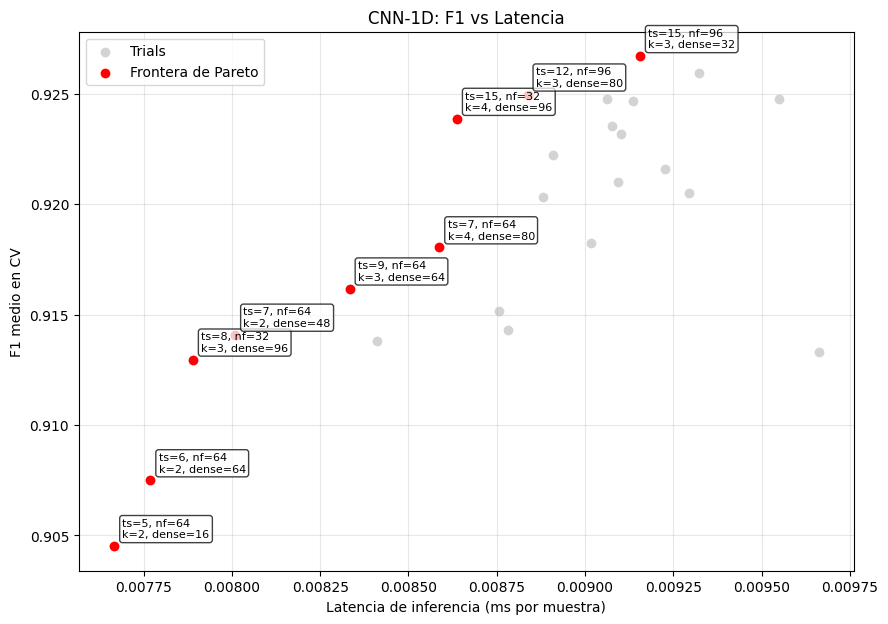
\includegraphics[width=0.8\textwidth]{images/PARETO_CNN.png}
    \caption{Frontera de Pareto - CNN}
    \label{fig:pareto_cnn}
\end{figure}

Los modelos seleccionados de la frontera de Pareto y sus resultados en el set de test son los siguientes:

\begin{table}[H]
    \centering
    \resizebox{\textwidth}{!}{% <-- Ajusta al ancho del texto
    \begin{tabular}{|l|c|c|c|c|c|c|c|}
        \hline
        \textbf{Perfil} & \textbf{n\_filters} & \textbf{kernel\_size} & \textbf{dense\_units} & \textbf{F1\_Test} & \textbf{Accuracy\_Test} & \textbf{Latencia (ms)} \\
        \hline
        Candidato 1 & 64 & 5 & 48 & 0.773052 & 0.793045 & 0.00888 \\
        \hline
        Candidato 2 & 128 & 5 & 64 & 0.761881 & 0.784118 & 0.009398 \\
        \hline
        Candidato 3 & 96 & 2 & 96 & 0.749724 & 0.77445 & 0.008625 \\
        \hline
        Candidato 4 & 32 & 5 & 16 & 0.738305 & 0.76551 & 0.008725 \\
        \hline
    \end{tabular}
    }
    \caption{Comparativa final de modelos CNN en el set de test}
    \label{tab:cnn_comparison}
\end{table}

El \textbf{Candidato 1} es el modelo ganador, con un F1-Score de 0.773052 y una latencia de inferencia de 0.00888 ms.
Aunque su rendimiento es excelente, su latencia es significativamente mayor que la de los modelos basados en árboles, lo que podría limitar su aplicabilidad en entornos de producción donde la velocidad de detección es crítica.


\section{Modelos entrenados con IoT-23}

\subsection{Random Forest}

Para el modelo de Random Forest, utilizando Optuna, se han obtenido los siguientes resultados como frontera de Pareto:

\begin{figure}[H]
    \centering
    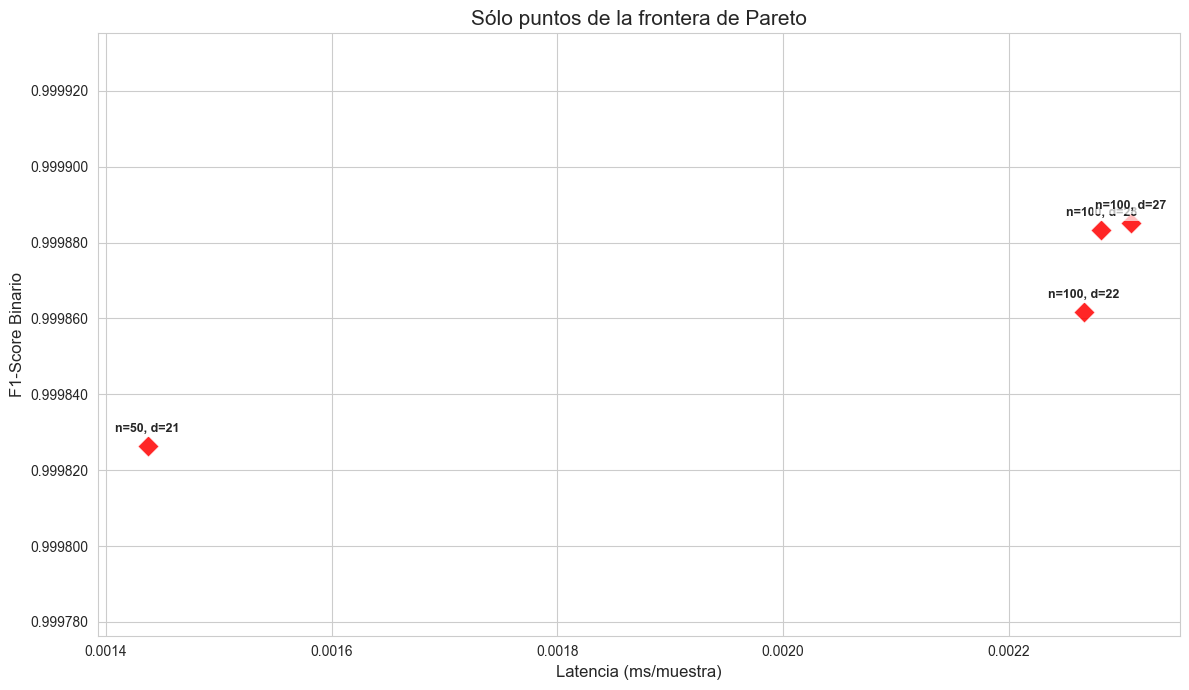
\includegraphics[width=0.8\textwidth]{images/IOT/PARETO_RF_IOT.png}
    \caption{Frontera de Pareto - Random Forest (IOT-23)}
    \label{fig:pareto_rf_iot}
\end{figure}

Hemos visto cómo reaccionan en test los modelos con los siguientes hiperparámetros elegidos:

\begin{enumerate}
    \item (50, 21) 
    \item (100, 22) 
    \item (100, 28) 
    \item (100, 27)
\end{enumerate}

Los resultados son los siguientes:

\begin{table}[H]
    \centering
    \begin{tabular}{|l|c|c|c|c|c|}
        \hline
        \textbf{Perfil} & \textbf{n\_estimators} & \textbf{max\_depth} & \textbf{F1\_Test} & \textbf{Accuracy\_Test} & \textbf{Latencia (ms)} \\
        \hline
        Candidato 1 & 50 & 21 & 0.999675 & 0.999614 & 0.001496 \\
        \hline
        Candidato 2 & 100 & 22 & 0.999855 & 0.999828 & 0.002252 \\
        \hline
        Candidato 3 & 100 & 28 & 0.999906 & 0.999888 & 0.002363 \\
        \hline
        Candidato 4 & 100 & 27 & 0.999913 & 0.999897 & 0.00223 \\
        \hline
    \end{tabular}
    \caption{Comparativa final de modelos Random Forest en el set de test (IOT-23)}
    \label{tab:rf_comparison_iot}
\end{table}

En este caso, el \textbf{Candidato 1} es el modelo más eficiente, con un F1-Score de 0.999675 y una latencia de inferencia de 0.001496 ms, lo que lo posiciona como un modelo extremadamente preciso y rápido para este dataset específico de IoT.

\subsection{XGBoost}

Para XGBoost, la frontera de Pareto obtenida es la siguiente:

\begin{figure}[H]
    \centering
    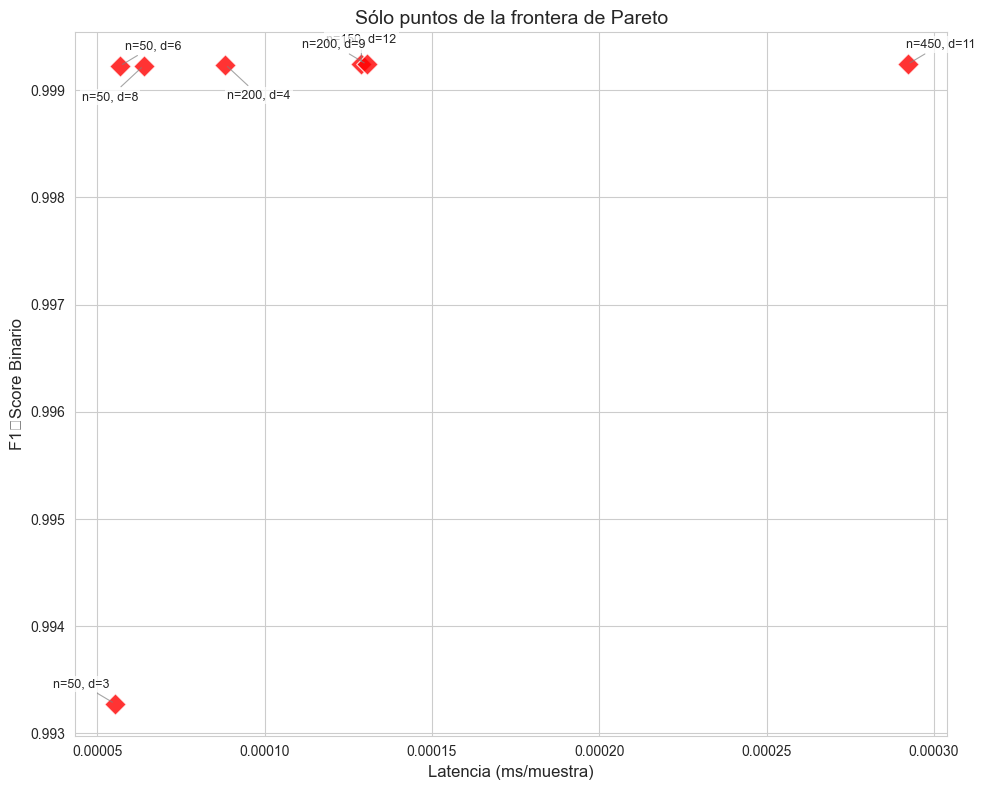
\includegraphics[width=0.8\textwidth]{images/IOT/PARETO_XGBOOST_IOT.png}
    \caption{Frontera de Pareto - XGBoost (IOT-23)}
    \label{fig:pareto_xgboost_iot}
\end{figure}

Los modelos seleccionados de la frontera de Pareto y sus resultados en el set de test son los siguientes:

\begin{enumerate}
    \item (50, 8) 
    \item (50, 6) 
    \item (200, 4) 
    \item (200, 9) 
    \item (150, 12)
\end{enumerate}

\begin{table}[H]
    \centering
    \begin{tabular}{|l|c|c|c|c|c|}
        \hline
        \textbf{Perfil} & \textbf{n\_estimators} & \textbf{max\_depth} & \textbf{F1\_Test} & \textbf{Accuracy\_Test} & \textbf{Latencia (ms)} \\
        \hline
        Candidato 1 & 50 & 8 & 0.999114 & 0.998948 & 0.000028 \\
        \hline
        Candidato 2 & 50 & 6 & 0.999122 & 0.998957 & 0.000027 \\
        \hline
        Candidato 3 & 200 & 4 & 0.999122 & 0.998957 & 0.000047 \\
        \hline
        Candidato 4 & 200 & 9 & 0.999132 & 0.998970 & 0.000080 \\
        \hline
        Candidato 5 & 150 & 12 & 0.999132 & 0.998970 & 0.000080 \\
        \hline
    \end{tabular}
    \caption{Comparativa final de modelos XGBoost en el set de test (IOT-23)}
    \label{tab:xgboost_comparison_iot}
\end{table}

En este caso, el \textbf{Candidato 2} es el modelo más eficiente, con un F1-Score de 0.999122 y una latencia de inferencia de 0.000027 ms, lo que lo posiciona como un modelo extremadamente preciso y rápido en este dataset de IoT, superando incluso a los modelos de Random Forest en términos de latencia.

\subsection{LightGBM}

La frontera de Pareto obtenida para LightGBM es la siguiente:

\begin{figure}[H]
    \centering
    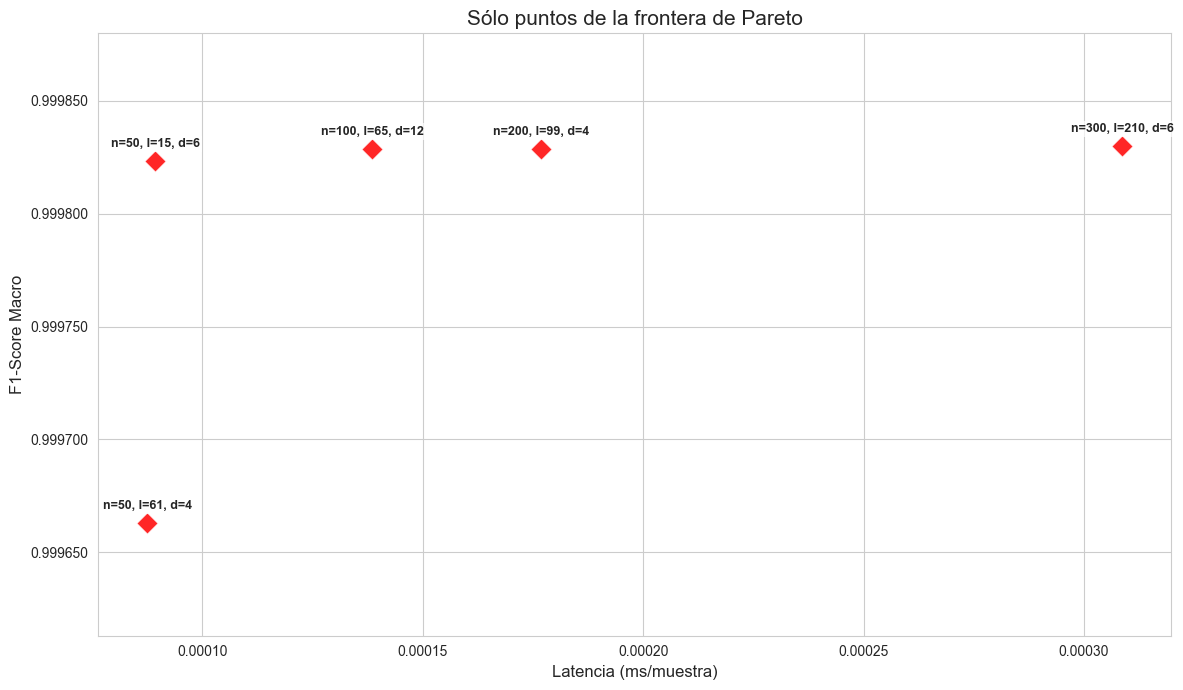
\includegraphics[width=0.8\textwidth]{images/IOT/PARETO_LIGHTGBM_IOT.png}
    \caption{Frontera de Pareto - LightGBM (IOT-23)}
    \label{fig:pareto_lightgbm_iot}
\end{figure}

Para este modelo, se han seleccionado los siguientes puntos de la frontera de Pareto para su evaluación en el set de test:

\begin{enumerate}
    \item (50, 15, 6) 
    \item (100, 65, 12) 
    \item (200, 99, 4) 
    \item (50, 61, 4) 
    \item (300, 210, 6) 
\end{enumerate}

Los resultados obtenidos en el set de test son los siguientes:

\begin{table}[H]
    \centering
    \begin{tabular}{|l|c|c|c|c|c|c|}
        \hline
        \textbf{Perfil} & \textbf{n\_estimators} & \textbf{num\_leaves} & \textbf{max\_depth} & \textbf{F1\_Test} & \textbf{Accuracy\_Test} & \textbf{Latencia (ms)} \\
        \hline
        Candidato 1 & 50 & 15 & 6 & 0.999813 & 0.99982 & 0.000057 \\
        \hline
        Candidato 2 & 100 & 65 & 12 & 0.999831 & 0.999837 & 0.000099 \\
        \hline
        Candidato 3 & 200 & 99 & 4 & 0.999795 & 0.999803 & 0.000170 \\
        \hline
        Candidato 4 & 50 & 61 & 4 & 0.999631 & 0.999644 & 0.000058 \\
        \hline
        Candidato 5 & 300 & 210 & 6 & 0.881924 & 0.882891 & 0.000261 \\
        \hline
    \end{tabular}
    \caption{Comparativa final de modelos LightGBM en el set de test (IOT-23)}
    \label{tab:lightgbm_comparison_iot}
\end{table}

En este caso, el \textbf{Candidato 1} es el mejor modelo, con un F1-Score de 0.999813 y una latencia de inferencia de 0.000057 ms, lo que lo posiciona como un modelo bastante bueno.

\subsection{CatBoost}

Este es el gráfico de la frontera de Pareto obtenida para CatBoost:

\begin{figure}[H]
    \centering
    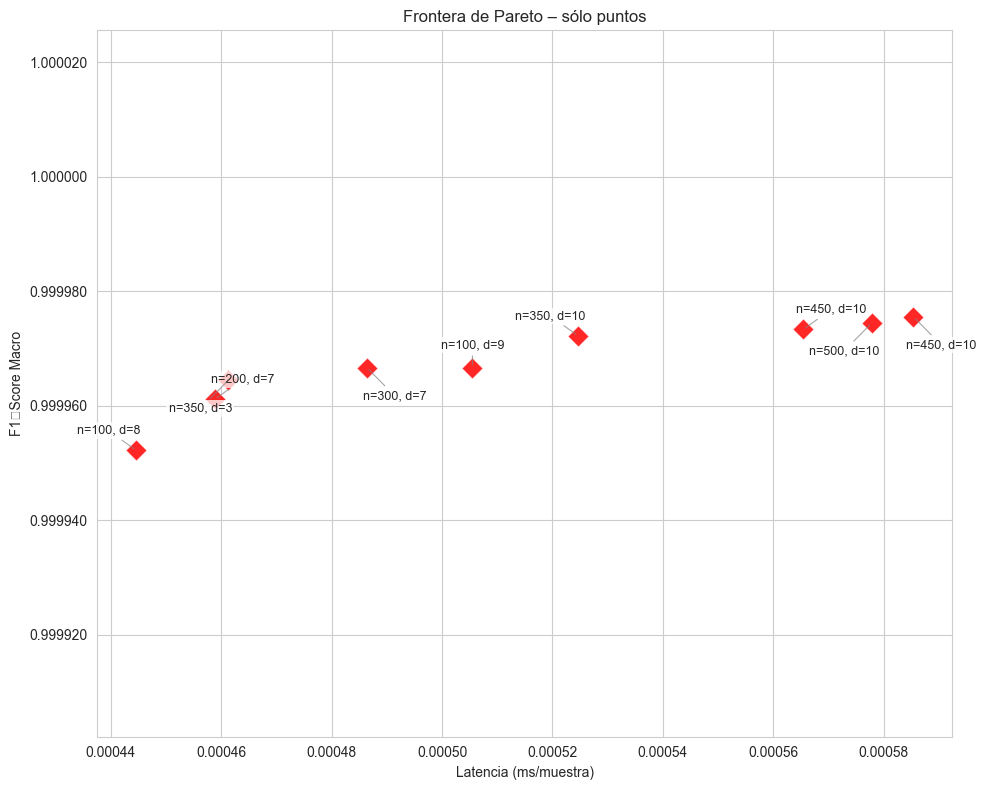
\includegraphics[width=0.8\textwidth]{images/IOT/PARETO_CATBOOST_IOT.png}
    \caption{Frontera de Pareto - CatBoost (IOT-23)}
    \label{fig:pareto_catboost_iot}
\end{figure}

Los modelos seleccionados de la frontera de Pareto y sus resultados en el set de test son los siguientes:

\begin{enumerate}
    \item (100, 8) 
    \item (350, 3) 
    \item (200, 7) 
    \item (300, 7) 
    \item (100, 9) 
    \item (350, 10) 
\end{enumerate}

\begin{table}[H]
    \centering
    \begin{tabular}{|l|c|c|c|c|c|}
        \hline
        \textbf{Perfil} & \textbf{n\_estimators} & \textbf{max\_depth} & \textbf{F1\_Test} & \textbf{Accuracy\_Test} & \textbf{Latencia (ms)} \\
        \hline
        Candidato 1 & 100 & 8 & 0.999947 & 0.999948 & 0.000242 \\
        \hline
        Candidato 2 & 350 & 3 & 0.999960 & 0.999961 & 0.000256 \\
        \hline
        Candidato 3 & 200 & 7 & 0.999951 & 0.999953 & 0.000263 \\
        \hline
        Candidato 4 & 300 & 7 & 0.999951 & 0.999953 & 0.000250 \\
        \hline
        Candidato 5 & 100 & 9 & 0.999951 & 0.999953 & 0.000259 \\
        \hline
        Candidato 6 & 350 & 10 & 0.999951 & 0.999953 & 0.000269 \\
        \hline
    \end{tabular}
    \caption{Comparativa final de modelos CatBoost en el set de test (IOT-23)}
    \label{tab:catboost_comparison_iot}
\end{table}

En este caso, el \textbf{Candidato 2} es el modelo más eficiente, con un F1-Score de 0.999960 y una latencia de inferencia de 0.000256 ms, lo que lo posiciona como un modelo extremadamente bueno.

\subsection{SVM}

La gráfica de la frontera de Pareto obtenida para SVM es la siguiente:

\begin{figure}[H]
    \centering
    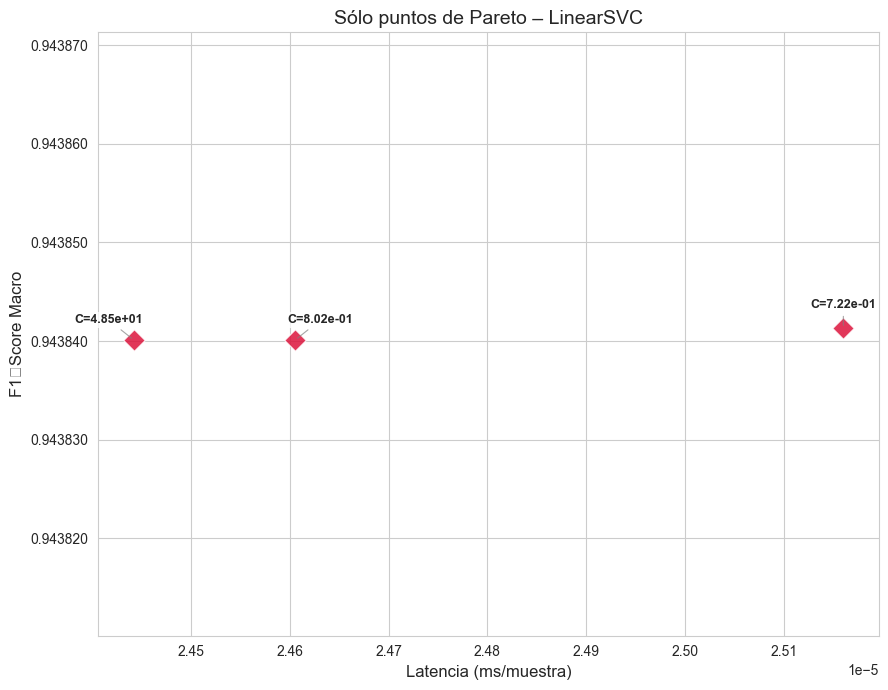
\includegraphics[width=0.8\textwidth]{images/IOT/PARETO_SVM_IOT.png}
    \caption{Frontera de Pareto - SVM (IOT-23)}
    \label{fig:pareto_svm_iot}
\end{figure}

Se han seleccionado los siguientes puntos de la frontera de Pareto para su evaluación en el set de test:

\begin{enumerate}
    \item (48.498258) 
    \item (0.801714) 
    \item (0.721883) 
\end{enumerate}

Los resultados obtenidos en el set de test para los modelos seleccionados de la frontera de Pareto son los siguientes:

\begin{table}[H]
    \centering
    \begin{tabular}{|l|c|c|c|c|}
        \hline
        \textbf{Perfil} & \textbf{C} & \textbf{F1\_Test} & \textbf{Accuracy\_Test} & \textbf{Latencia (ms)} \\
        \hline
        Candidato 1 & 48.498258 & 0.943691 & 0.945963 & 0.000027 \\
        \hline
        Candidato 2 & 0.801714 & 0.943695 & 0.945968 & 0.000025 \\
        \hline
        Candidato 3 & 0.721883 & 0.943691 & 0.945963 & 0.000023 \\
        \hline
    \end{tabular}
    \caption{Comparativa final de modelos SVM en el set de test (IOT-23)}
    \label{tab:svm_comparison_iot}
\end{table}

En este caso, el \textbf{Candidato 2} es el modelo más eficiente, con un F1-Score de 0.943695 y una latencia de inferencia de 0.000025 ms, lo que lo posiciona como un modelo muy bueno para este dataset de IoT, aunque su rendimiento es significativamente inferior al de los modelos basados en árboles.

\subsection{MLP}

La gráfica de la frontera de Pareto obtenida para MLP es la siguiente:

\begin{figure}[H]
    \centering
    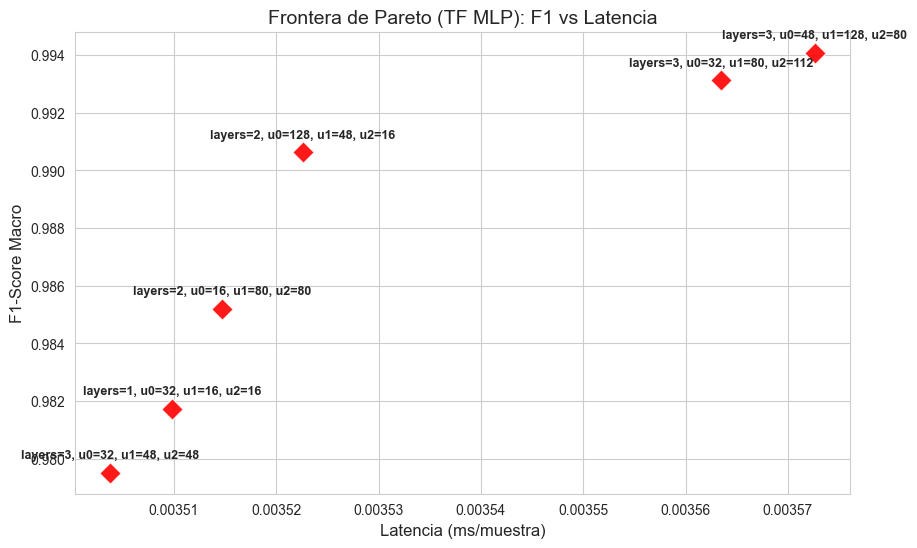
\includegraphics[width=0.8\textwidth]{images/IOT/PARETO_MLP_IOT.png}
    \caption{Frontera de Pareto - MLP (IOT-23)}
    \label{fig:pareto_mlp_iot}
\end{figure}

La combinación de hiperparámetros seleccionada para su evaluación en el set de test es la siguiente:

\begin{enumerate}
    \item (3, 32, 48, 48) 
    \item (1, 32, 0, 0) 
    \item (2, 16, 80, 0) 
    \item (2, 128, 48, 0) 
    \item (3, 32, 80, 112) 
    \item (3, 48, 128, 80) 
\end{enumerate}

Los resultados obtenidos en el set de test para los modelos seleccionados de la frontera de Pareto son los siguientes:

\begin{table}[H]
    \centering
    \resizebox{\textwidth}{!}{
    \begin{tabular}{|l|c|c|c|c|c|c|c|}
        \hline
        \textbf{Perfil} & \textbf{n\_layers} & \textbf{n\_units\_l0} & \textbf{n\_units\_l1} & \textbf{n\_units\_l2} & \textbf{F1\_Test} & \textbf{Accuracy\_Test} & \textbf{Latencia (ms)} \\
        \hline
        Candidato 1 & 3 & 32 & 48 & 48 & 0.994819 & 0.995004 & 0.000717 \\
        \hline
        Candidato 2 & 1 & 32 & 0 & 0 & 0.985158 & 0.985741 & 0.000621 \\
        \hline
        Candidato 3 & 2 & 16 & 80 & 0 & 0.990610 & 0.990969 & 0.000719 \\
        \hline
        Candidato 4 & 2 & 128 & 48 & 0 & 0.993502 & 0.993737 & 0.000772 \\
        \hline
        Candidato 5 & 3 & 32 & 80 & 112 & 0.995042 & 0.995223 & 0.000919 \\
        \hline
        Candidato 6 & 3 & 48 & 128 & 80 & 0.996544 & 0.996665 & 0.000906 \\
        \hline
    \end{tabular}
    }
    \caption{Comparativa final de modelos MLP en el set de test (IOT-23)}
    \label{tab:mlp_comparison_iot}
\end{table}

En este caso, nos quedamos con el \textbf{Candidato 1}, que ofrece un excelente rendimiento (F1-Score de 0.994819) y una latencia de inferencia de 0.000717 ms, lo que lo posiciona como un modelo muy bueno para este dataset de IoT, aunque su rendimiento sigue siendo inferior al de los modelos basados en árboles.

\subsection{CNN-1D}

La gráfica de la frontera de Pareto obtenida para CNN-1D es la siguiente:

\begin{figure}[H]
    \centering
    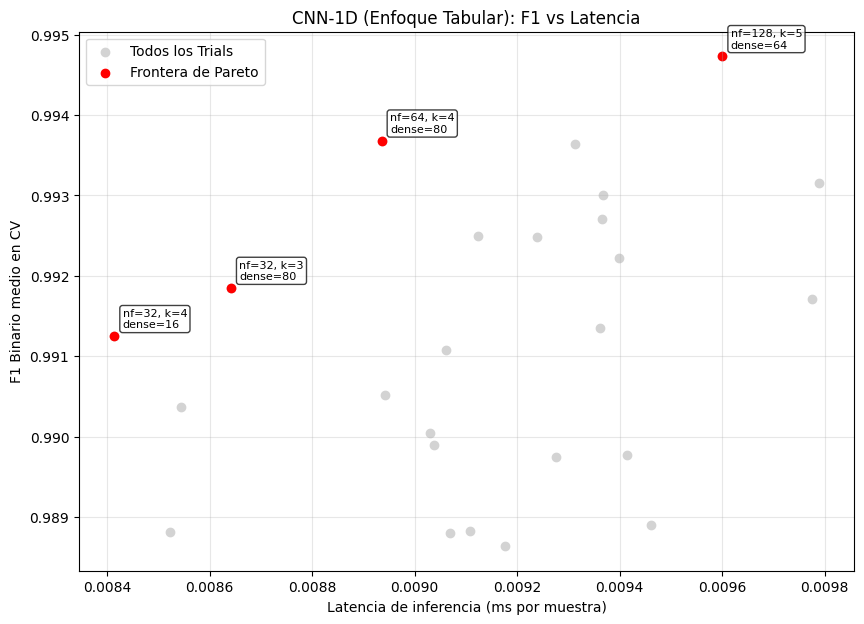
\includegraphics[width=0.8\textwidth]{images/IOT/PARETO_CNN_IOT.png}
    \caption{Frontera de Pareto - CNN-1D (IOT-23)}
    \label{fig:pareto_cnn_iot}
\end{figure}

Los modelos seleccionados de la frontera de Pareto y sus resultados en el set de test son los siguientes:

\begin{enumerate}
    \item (32, 4, 16) 
    \item (32, 3, 80) 
    \item (64, 4, 80) 
    \item (128, 5, 64) 
\end{enumerate} 

\begin{table}[H]
    \centering
    \begin{tabular}{|l|c|c|c|c|c|c|}
        \hline
        \textbf{Perfil} & \textbf{n\_filters} & \textbf{kernel\_size} & \textbf{dense\_units} & \textbf{F1\_Test} & \textbf{Accuracy\_Test} & \textbf{Latencia (ms)} \\
        \hline
        Candidato 1 & 32 & 4 & 16 & 0.992844 & 0.991467 & 0.008293 \\
        \hline
        Candidato 2 & 32 & 3 & 80 & 0.988798 & 0.986561 & 0.008442 \\
        \hline
        Candidato 3 & 64 & 4 & 80 & 0.995359 & 0.99448 & 0.00892 \\
        \hline
        Candidato 4 & 128 & 5 & 64 & 0.99583 & 0.995042 & 0.009345 \\
        \hline
    \end{tabular}
    \caption{Comparativa final de modelos CNN-1D en el set de test (IOT-23)}
    \label{tab:cnn_comparison_iot}
\end{table}

En este caso, el \textbf{Candidato 3} es el modelo más eficiente, con un F1-Score de 0.995359 y una latencia de inferencia de 0.00892 ms, lo que lo posiciona como un modelo muy bueno para este dataset de IoT, aunque su rendimiento sigue siendo inferior al de los modelos basados en árboles.

\section{Modelos entrenados con TON-IoT}

\subsection{Random Forest}

La frontera de Pareto obtenida para Random Forest con el dataset ToN-IoT es la siguiente:

\begin{figure}[H]
    \centering
    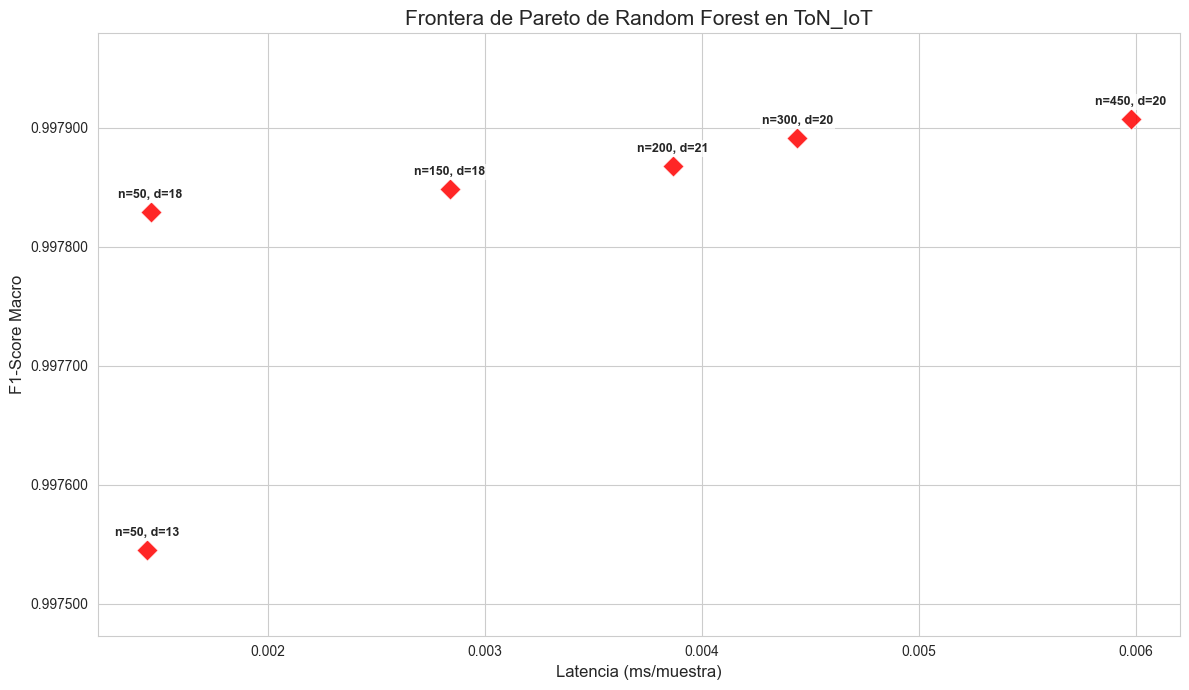
\includegraphics[width=0.8\textwidth]{images/TON/PARETO_RF_TON.png}
    \caption{Frontera de Pareto - Random Forest (ToN-IoT)}
    \label{fig:pareto_rf_ton}
\end{figure}

Los modelos seleccionados de la frontera de Pareto y sus resultados en el set de test son los siguientes:
\begin{enumerate}
    \item (50, 13) 
    \item (50, 18) 
    \item (150, 18) 
    \item (200, 21)
    \item (300, 20)
    \item (450, 20)
\end{enumerate}

\begin{table}[H]
    \centering
    \begin{tabular}{|l|c|c|c|c|c|}
        \hline
        \textbf{Perfil} & \textbf{n\_estimators} & \textbf{max\_depth} & \textbf{F1\_Test} & \textbf{Accuracy\_Test} & \textbf{Latencia (ms)} \\
        \hline
        Candidato 1 & 50 & 13 & 0.995912 & 0.997039 & 0.001468 \\
        \hline
        Candidato 2 & 50 & 18 & 0.996434 & 0.997418 & 0.001459 \\
        \hline
        Candidato 3 & 150 & 18 & 0.996369 & 0.99737 & 0.002886 \\
        \hline
        Candidato 4 & 200 & 21 & 0.996598 & 0.997536 & 0.004955 \\
        \hline
        Candidato 5 & 300 & 20 & 0.996271 & 0.997299 & 0.004452 \\
        \hline
        Candidato 6 & 450 & 20 & 0.996369 & 0.99737 & 0.00759 \\
        \hline
    \end{tabular}
    \caption{Comparativa final de modelos Random Forest en el set de test (ToN-IoT)}
    \label{tab:rf_comparison_ton}
\end{table}

El \textbf{Candidato 2} representa el punto de equilibrio perfecto (el óptimo de Pareto) entre capacidad de detección y coste computacional.

\subsection{XGBoost}

La frontera de Pareto obtenida para XGBoost con el dataset ToN-IoT es la siguiente:

\begin{figure}[H]
    \centering
    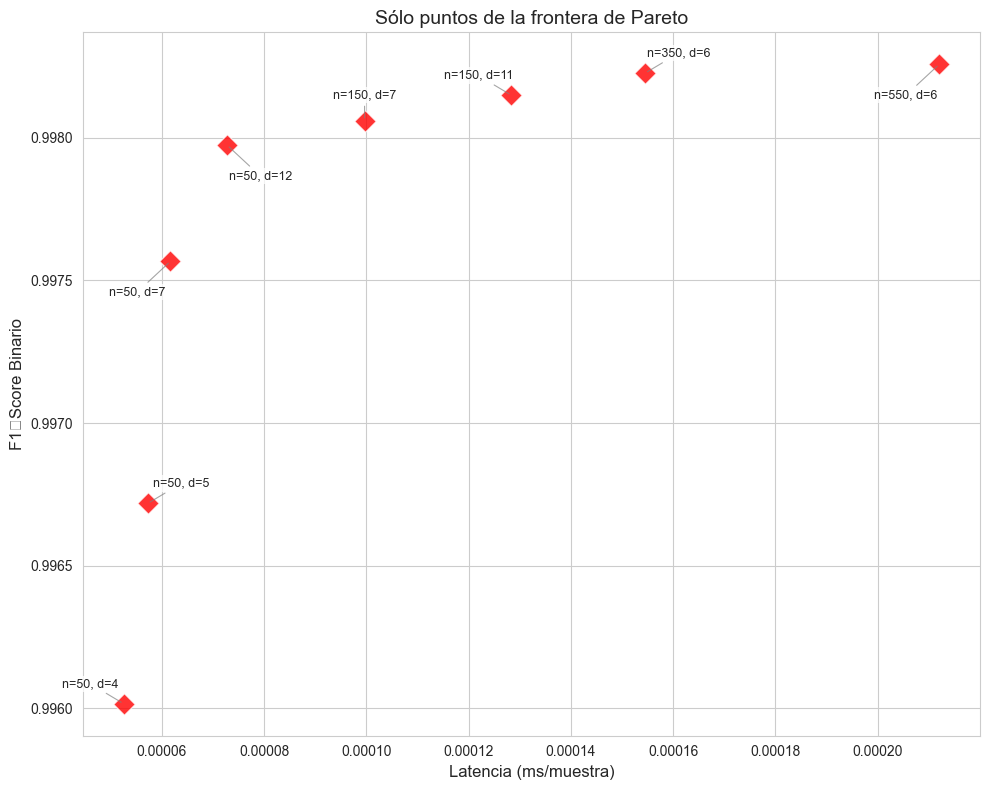
\includegraphics[width=0.8\textwidth]{images/TON/PARETO_XGBOOST_TON.png}
    \caption{Frontera de Pareto - XGBoost (ToN-IoT)}
    \label{fig:pareto_xgboost_ton}
\end{figure}

Los modelos seleccionados de la frontera de Pareto y sus resultados en el set de test son los siguientes:

\begin{enumerate}
    \item (50, 4) 
    \item (50, 5) 
    \item (50, 7) 
    \item (50, 12) 
    \item (150, 7) 
    \item (150, 11) 
    \item (350, 6)
    \item (550, 6)
\end{enumerate}

\begin{table}[H]
    \centering
    \begin{tabular}{|l|c|c|c|c|c|}
        \hline
        \textbf{Perfil} & \textbf{n\_estimators} & \textbf{max\_depth} & \textbf{F1\_Test} & \textbf{Accuracy\_Test} & \textbf{Latencia (ms)} \\
        \hline
        Candidato 1 & 50 & 4 & 0.995979 & 0.993864 & 0.00005 \\
        \hline
        Candidato 2 & 50 & 5 & 0.99713 & 0.995617 & 0.000039 \\
        \hline
        Candidato 3 & 50 & 7 & 0.997734 & 0.996541 & 0.000042 \\
        \hline
        Candidato 4 & 50 & 12 & 0.998168 & 0.997204 & 0.000071 \\
        \hline
        Candidato 5 & 150 & 7 & 0.998231 & 0.997299 & 0.000071 \\
        \hline
        Candidato 6 & 150 & 11 & 0.998246 & 0.997323 & 0.000096 \\
        \hline
        Candidato 7 & 350 & 6 & 0.998261 & 0.997347 & 0.000116 \\
        \hline
        Candidato 8 & 550 & 6 & 0.99823 & 0.997299 & 0.000167 \\
        \hline
    \end{tabular}
    \caption{Comparativa final de modelos XGBoost en el set de test (ToN-IoT)}
    \label{tab:xgboost_comparison_ton}
\end{table}

Vamos a seleccionar al \textbf{Candidato 3} ya que representa un compromiso perfecto entre capacidad de detección y coste computacional, con un F1-Score de 0.997734 y una latencia de inferencia de 0.000042 ms.

\subsection{LightGBM}

La frontera de Pareto obtenida para LightGBM con el dataset ToN-IoT es la siguiente:

\begin{figure}[H]
    \centering
    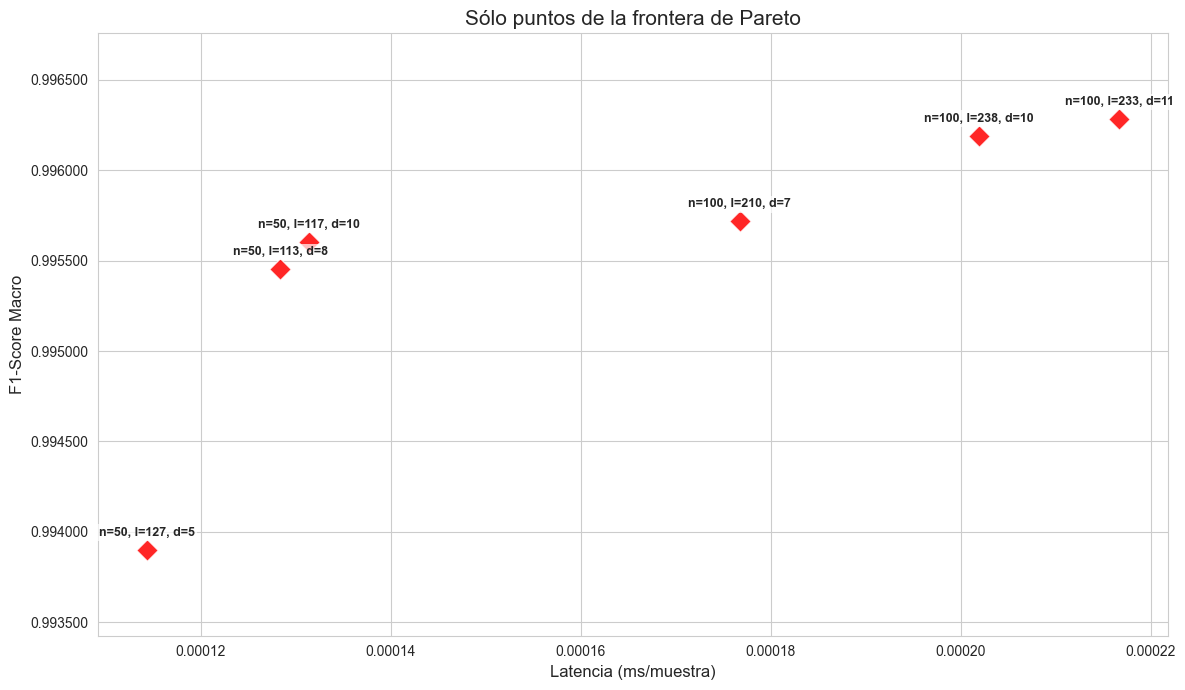
\includegraphics[width=0.8\textwidth]{images/TON/PARETO_LIGHTGBM_TON.png}
    \caption{Frontera de Pareto - LightGBM (ToN-IoT)}
    \label{fig:pareto_lightgbm_ton}
\end{figure}

Los modelos seleccionados de la frontera de Pareto y sus resultados en el set de test son los siguientes:

\begin{enumerate}
    \item (50, 127, 5) 
    \item (50, 113, 8) 
    \item (50, 117, 10) 
    \item (100, 210, 7) 
    \item (100, 238, 10) 
    \item (100, 233, 11)
\end{enumerate}

\begin{table}[H]
    \centering
    \begin{tabular}{|l|c|c|c|c|c|c|}
        \hline
        \textbf{Perfil} & \textbf{n\_estimators} & \textbf{num\_leaves} & \textbf{max\_depth} & \textbf{F1\_Test} & \textbf{Accuracy\_Test} & \textbf{Latencia (ms)} \\
        \hline
        Candidato 1 & 50 & 127 & 5 & 0.99456 & 0.996067 & 0.00011 \\
        \hline
        Candidato 2 & 50 & 113 & 8 & 0.996134 & 0.997204 & 0.000113 \\
        \hline
        Candidato 3 & 50 & 117 & 10 & 0.996299 & 0.997323 & 0.000298 \\
        \hline
        Candidato 4 & 100 & 210 & 7 & 0.996594 & 0.997536 & 0.000181 \\
        \hline
        Candidato 5 & 100 & 238 & 10 & 0.996955 & 0.997797 & 0.000191 \\
        \hline
        Candidato 6 & 100 & 233 & 11 & 0.997085 & 0.997891 & 0.000202 \\
        \hline
    \end{tabular}
    \caption{Comparativa final de modelos LightGBM en el set de test (ToN-IoT)}
    \label{tab:lightgbm_comparison_ton}
\end{table}

Nos quedamos con el \textbf{Candidato 6} que ofrece un excelente rendimiento (F1-Score de 0.997085) y una latencia de inferencia de 0.000202 ms, lo que lo posiciona como un modelo muy bueno para este dataset de IoT, aunque su rendimiento sigue siendo inferior al de los modelos basados en árboles.

\subsection{CatBoost}

Para CatBoost, la frontera de Pareto obtenida con el dataset ToN-IoT es la siguiente:

\begin{figure}[H]
    \centering
    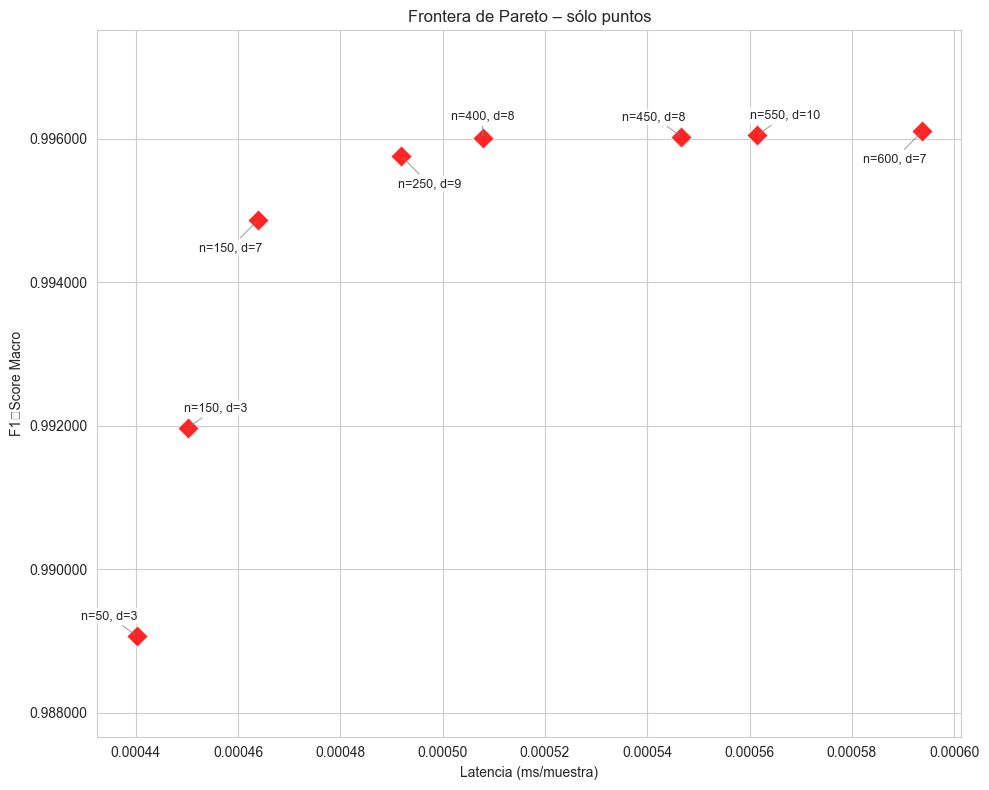
\includegraphics[width=0.8\textwidth]{images/TON/PARETO_CATBOOST_TON.png}
    \caption{Frontera de Pareto - CatBoost (ToN-IoT)}
    \label{fig:pareto_catboost_ton}
\end{figure}

Los modelos seleccionados de la frontera de Pareto y sus resultados en el set de test son los siguientes:

\begin{enumerate}
    \item (50, 3) 
    \item (150, 3) 
    \item (150, 7) 
    \item (250, 9) 
    \item (400, 8) 
    \item (450, 8) 
    \item (550, 10) 
    \item (600, 7) 
\end{enumerate}

\begin{table}[H]
    \centering
    \begin{tabular}{|l|c|c|c|c|c|}
        \hline
        \textbf{Perfil} & \textbf{n\_estimators} & \textbf{max\_depth} & \textbf{F1\_Test} & \textbf{Accuracy\_Test} & \textbf{Latencia (ms)} \\
        \hline
        Candidato 1 & 50 & 3 & 0.98919 & 0.992205 & 0.000274 \\
        \hline
        Candidato 2 & 150 & 3 & 0.992427 & 0.994527 & 0.00031 \\
        \hline
        Candidato 3 & 150 & 7 & 0.995842 & 0.996991 & 0.00033 \\
        \hline
        Candidato 4 & 250 & 9 & 0.996628 & 0.99756 & 0.000354 \\
        \hline
        Candidato 5 & 400 & 8 & 0.996726 & 0.997631 & 0.000456 \\
        \hline
        Candidato 6 & 450 & 8 & 0.996758 & 0.997655 & 0.00057 \\
        \hline
        Candidato 7 & 550 & 10 & 0.996759 & 0.997655 & 0.000461 \\
        \hline
        Candidato 8 & 600 & 7 & 0.996792 & 0.997678 & 0.000419 \\
        \hline
    \end{tabular}
    \caption{Comparativa final de modelos CatBoost en el set de test (ToN-IoT)}
    \label{tab:catboost_comparison_ton}
\end{table}

El \textbf{Candidato 4} representa el punto de equilibrio perfecto (el óptimo de Pareto) entre capacidad de detección y coste computacional, con un F1-Score de 0.996628 y una latencia de inferencia de 0.000354 ms.

\subsection{SVM}

La frontera de Pareto obtenida para SVM con el dataset ToN-IoT es la siguiente:

\begin{figure}[H]
    \centering
    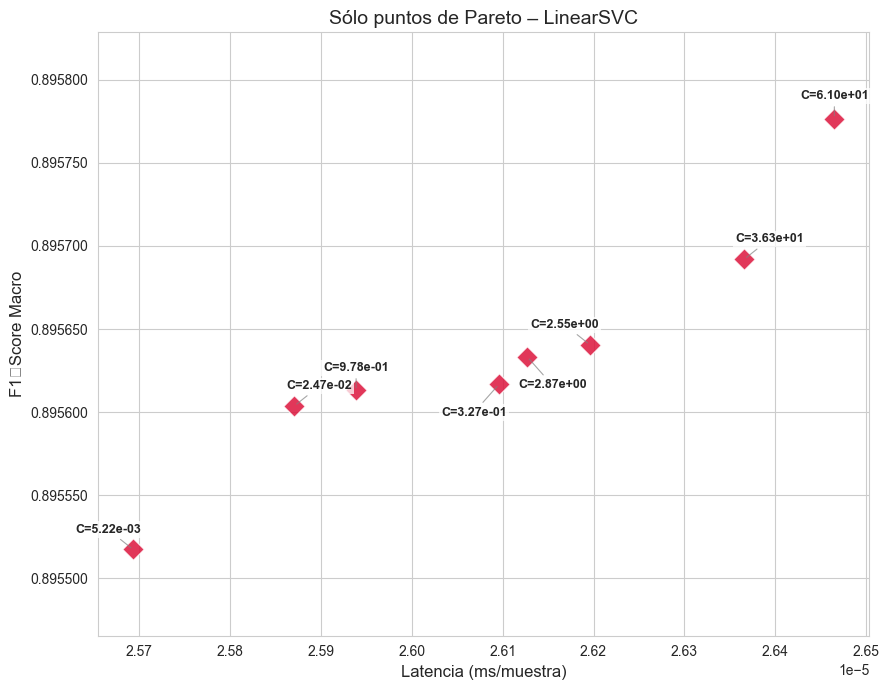
\includegraphics[width=0.8\textwidth]{images/TON/PARETO_SVM_TON.png}
    \caption{Frontera de Pareto - SVM (ToN-IoT)}
    \label{fig:pareto_svm_ton}
\end{figure}

Los candidatos seleccionados de la frontera de Pareto son:

\begin{enumerate}
    \item (0.024697) 
    \item (0.977892) 
    \item (0.326653) 
    \item (2.870875) 
    \item (2.552291) 
    \item (36.274336) 
\end{enumerate}

Los resultados obtenidos en el set de test para los modelos seleccionados de la frontera de Pareto son los siguientes:

\begin{table}[H]
    \centering
    \begin{tabular}{|l|c|c|c|c|}
        \hline
        \textbf{Perfil} & \textbf{C} & \textbf{F1\_Test} & \textbf{Accuracy\_Test} & \textbf{Latencia (ms)} \\
        \hline
        Candidato 1 & 0.024697 & 0.897624 & 0.926603 & 0.000027 \\
        \hline
        Candidato 2 & 0.977892 & 0.897712 & 0.926674 & 0.000051 \\
        \hline
        Candidato 3 & 0.326653 & 0.897712 & 0.926674 & 0.000029 \\
        \hline
        Candidato 4 & 2.870875 & 0.897815 & 0.926745 & 0.000031 \\
        \hline
        Candidato 5 & 2.552291 & 0.897712 & 0.926674 & 0.000047 \\
        \hline
        Candidato 6 & 36.274336 & 0.897785 & 0.926722 & 0.000029 \\
        \hline
    \end{tabular}
    \caption{Comparativa final de modelos SVM en el set de test (ToN-IoT)}
    \label{tab:svm_comparison_ton}
\end{table}

El \textbf{Candidato 4} representa el punto de equilibrio perfecto (el óptimo de Pareto) entre capacidad de detección y coste computacional, con un F1-Score de 0.897815 y una latencia de inferencia de 0.000031 ms, lo que lo posiciona como un modelo bastante bueno para este dataset de IoT, aunque su rendimiento es significativamente inferior al de los modelos basados en árboles.

\subsection{MLP}

La frontera de Pareto obtenida para MLP con el dataset ToN-IoT es la siguiente:

\begin{figure}[H]
    \centering
    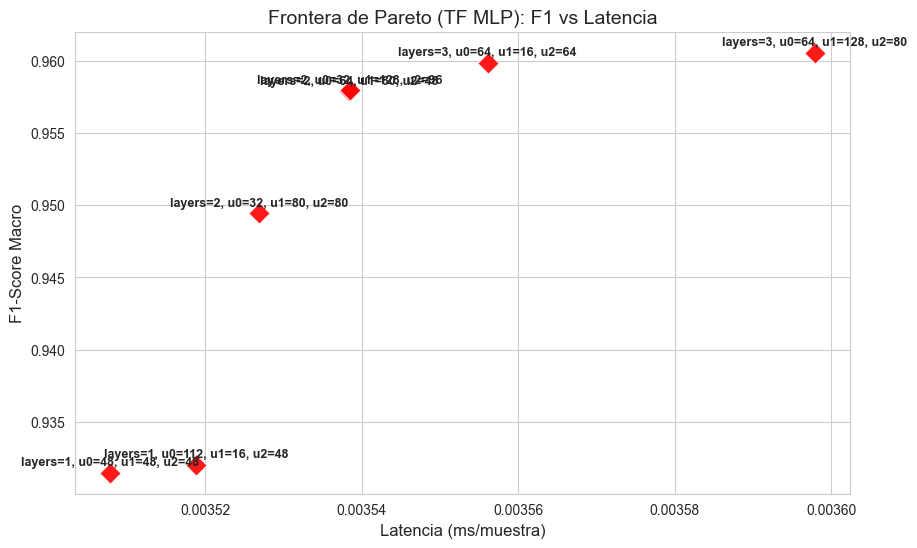
\includegraphics[width=0.8\textwidth]{images/TON/PARETO_MLP_TON.png}
    \caption{Frontera de Pareto - MLP (ToN-IoT)}
    \label{fig:pareto_mlp_ton}
\end{figure}

Los modelos seleccionados de la frontera de Pareto y sus resultados en el set de test son los siguientes:

\begin{enumerate}
    \item (2, 32, 80, 0) 
    \item (2, 64, 80, 0) 
    \item (2, 32, 128, 0) 
    \item (3, 64, 16, 64) 
\end{enumerate}

\begin{table}[H]
    \centering
    \small
    \setlength{\tabcolsep}{3pt}
    \begin{tabular}{|l|c|c|c|c|c|c|c|}
        \hline
        \textbf{Perfil} & \textbf{Capas} & \textbf{U. l0} & \textbf{U. l1} & \textbf{U. l2} & \textbf{F1} & \textbf{Accuracy} & \textbf{Lat. (ms)} \\
        \hline
        Candidato 1 & 2 & 32 & 80 & 0 & 0.961973 & 0.9733 & 0.002257 \\
        \hline
        Candidato 2 & 2 & 64 & 80 & 0 & 0.962048 & 0.973418 & 0.002328 \\
        \hline
        Candidato 3 & 2 & 32 & 128 & 0 & 0.96124 & 0.972873 & 0.00237 \\
        \hline
        Candidato 4 & 3 & 64 & 16 & 64 & 0.963034 & 0.97401 & 0.002268 \\
        \hline
    \end{tabular}
    \caption{Comparativa final de modelos MLP en el set de test (ToN-IoT)}
    \label{tab:mlp_comparison_ton}
\end{table}

El \textbf{Candidato 4} representa el punto de equilibrio perfecto (el óptimo de Pareto) entre capacidad de detección y coste computacional, con un F1-Score de 0.963034 y una latencia de inferencia de 0.002268 ms, lo que lo posiciona como un modelo bastante bueno para este dataset de IoT, aunque su rendimiento sigue siendo inferior al de los modelos basados en árboles.

\subsection{CNN-1D}

La frontera de Pareto obtenida para CNN-1D con el dataset ToN-IoT es la siguiente:

\begin{figure}[H]
    \centering
    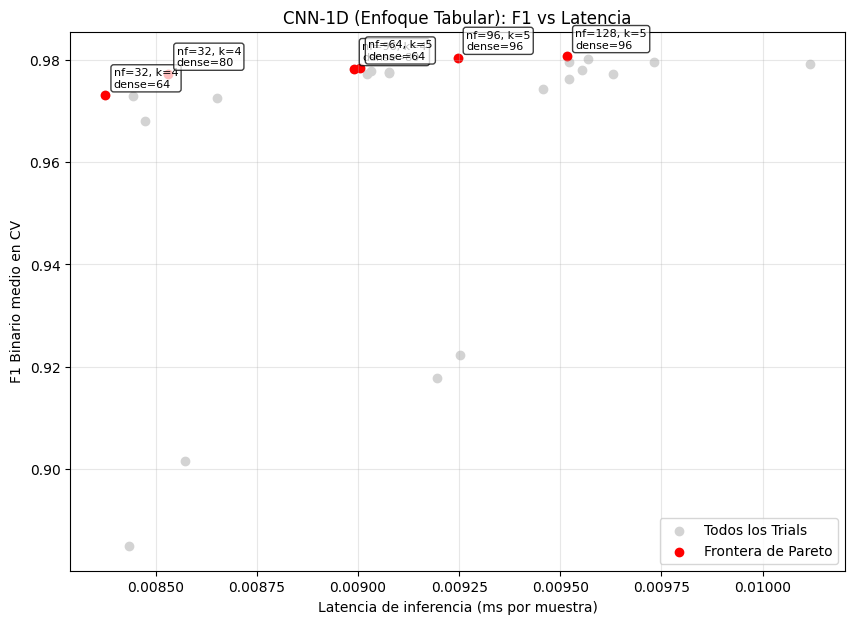
\includegraphics[width=0.8\textwidth]{images/TON/PARETO_CNN_TON.png}
    \caption{Frontera de Pareto - CNN-1D (ToN-IoT)}
    \label{fig:pareto_cnn_ton}
\end{figure}

Los modelos seleccionados de la frontera de Pareto y sus resultados en el set de test son los siguientes:

\begin{enumerate}
    \item (32, 4, 64) 
    \item (32, 4, 80) 
    \item (96, 4, 80) 
    \item (64, 5, 64) 
    \item (96, 5, 96) 
    \item (128, 5, 96) 
\end{enumerate}

\begin{table}[H]
    \centering
    \begin{tabular}{|l|c|c|c|c|c|c|}
        \hline
        \textbf{Perfil} & \textbf{n\_filters} & \textbf{kernel\_size} & \textbf{dense\_units} & \textbf{F1\_Test} & \textbf{Accuracy\_Test} & \textbf{Latencia (ms)} \\
        \hline
        Candidato 1 & 32 & 4 & 64 & 0.977894 & 0.96586 & 0.008596 \\
        \hline
        Candidato 2 & 32 & 4 & 80 & 0.974993 & 0.96124 & 0.009421 \\
        \hline
        Candidato 3 & 96 & 4 & 80 & 0.978447 & 0.966737 & 0.009012 \\
        \hline
        Candidato 4 & 64 & 5 & 64 & 0.981183 & 0.970836 & 0.009133 \\
        \hline
        Candidato 5 & 96 & 5 & 96 & 0.981769 & 0.97176 & 0.008953 \\
        \hline
        Candidato 6 & 128 & 5 & 96 & 0.981696 & 0.971641 & 0.009564 \\
        \hline
    \end{tabular}
    \caption{Comparativa final de modelos CNN-1D en el set de test (ToN-IoT)}
    \label{tab:cnn_comparison_ton}
\end{table}

El ganador es el \textbf{Candidato 5} que ofrece el rendimiento más alto (F1-Score de 0.981769) y una latencia de inferencia de 0.008953 ms.
